\subsection{MetaPath}

In the previous MetaDE package,
pathway analysis is performed using the declared DE genes from MetaDE analysis.
The MetaPath module  performs pathway analysis by two advanced meta-analytic pathway analysis tools: 
Meta-Analysis for Pathway Enrichment (MAPE) and Comparative Pathway Integrator (CPI) (Shen et al., 2010; Fang et al., 2017). 
Instead of directly using the declared DE genes from MetaDE analysis as input, 
the MAPE algorithm performs pathway analysis in each study and performs meta-analysis on the pathway level.
%Pathway clustering with statistically valid text mining is included in the package to reduce pathway redundancy to condense knowledge and increase interpretability of clustering results. 
In addition, CPI also includes advanced pathway clustering diagnostics and pathway clustering with text mining to circumvent abundant pathway redundancy in the databases and improve interpretation. 
The R package for MetaPath module can be found at \url{https://github.com/metaOmics/MetaPath}.

Note that both MetaDE and MetaPath could perform pathway enrichment analysis.
Below are their differences.
MetaDE only provides more traditional downstream pathway analysis for the functional annotation of detected DE genes from meta-analysis. On the other hand, MetaPath uses more comprehensive and sophisticated methods to jointly perform DE analysis and pathway analysis, 
and it provides stronger statistical power and more extensive and intuitive biological insights. 
For example, MAPE\_G is more similar to MetaDE in a sense since both of them combine gene level p-values first and then perform pathway analysis, while MAPE\_P is different since it performs single-study DE and pathway analysis first and then combines pathway level p-values. 
MAPE\_I takes the advantage of both, 
and CPI is a more advanced algorithm to further perform meta-analysis on studies with known heterogeneities. In addition, MetaPath performs additional pathway clustering to reduce pathway redundancy and extracts the key words from each cluster via the text mining algorithm to assist with the interpretation. 

\subsubsection{Procedure}
The MetaPath package requires the input of raw expression data as in MetaDE. 
There are three major steps to implement the package: pathway analysis, pathway clustering diagnostics, 
and pathway clustering with text mining. 
As shown in Figure \ref{fig:MetaPathoption}, there are nine major options that need to be specified to implement the package.
A complete list of all options for the package can be found in Section~\ref{sec:completeList_MetaPath} 


\begin{figure}[H]
\begin{center}
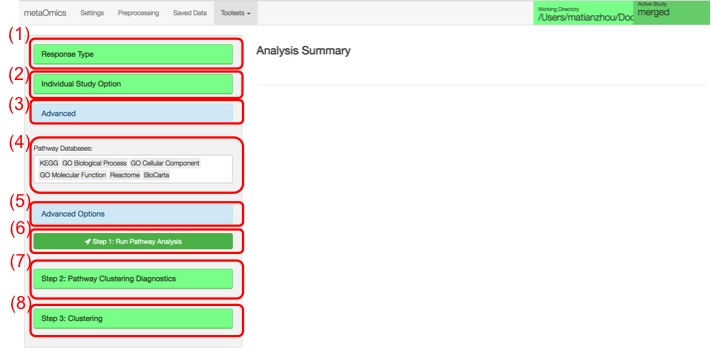
\includegraphics[scale=0.5]{./figure/metaPath/metaPathoption.pdf}
\caption{MetaPath options}
\label{fig:MetaPathoption}
\end{center}
\end{figure}

\textbf{Setup pathway analysis parameters:}
As shown in Figure~\ref{fig:MetaPathoption},
users need to specify {\color{red}(1)} whether the input gene-expression profile is a mix of continuous data and discrete data;
{\color{red}(2)} response type, case/control labels (similar to MetaDE);
{\color{red}(3)} individual study option (similar to MetaDE);
{\color{red}(4)} advanced options, including whether to adjust for covariates or the direction of hypothesis testing.
In {\color{red}(5)}, users can select from 25 available pathway databases for the enrichment analysis.
In {\color{red}(6)}, users can select the MetaPath method (either MAPE or CPI).
By default, the MAPE approach is used. 
Other options include the pathway enrichment method (Fisher's Exact Test or KS Test), 
the minimum and maximum pathway size. If Fisher's exact test is chosen for the enrichment method, users need to further specify the criteria for selection of DE genes, (e.g., the number of top ranked genes). 
On the other hand, if KS test is chosen, one needs to further specify whether to use permutation to obtain the enrichment p-value. 

\begin{steps}
\item \textbf{Run pathway analysis:}
\label{step:metaPath1}
Once the above options are specified, users can click on {\color{red}(7)} to ``Run Pathway Analysis".

\item \textbf{Pathway clustering diagnostics:} 
\label{step:metaPath2}
Since these pathways may contain redundant information, 
we want to cluster these pathways into certain groups. 
The first thing is to determine number of clusters $K$.
Following the previous step (\ref{step:metaPath1}), 
users can specify the top enriched pathways for further clustering. 
The top enriched pathways can be specified by choosing the FDR cutoff by expanding the drop-down menu in {\color{red}(8)}.
Then, by clicking on ``Pathway Clustering Diagnostics" (Figure~\ref{fig:MetaPathoption} {\color{red}(8)}),
the MetaPath module will perform consensus clustering analysis to determine the optimum number of clusters $K$.


\item \textbf{Pathway clustering with text mining:} 
\label{step:metaPath3}
From the previous step (\ref{step:metaPath2}), users can determine the optimal number of clusters in the pool of pathways selected. 
Now, one can specify the number of clusters and click on {\color{red}(9)} to get pathway clustering results. 
\end{steps}




\subsubsection{Results}

\begin{figure}[H]
\begin{center}
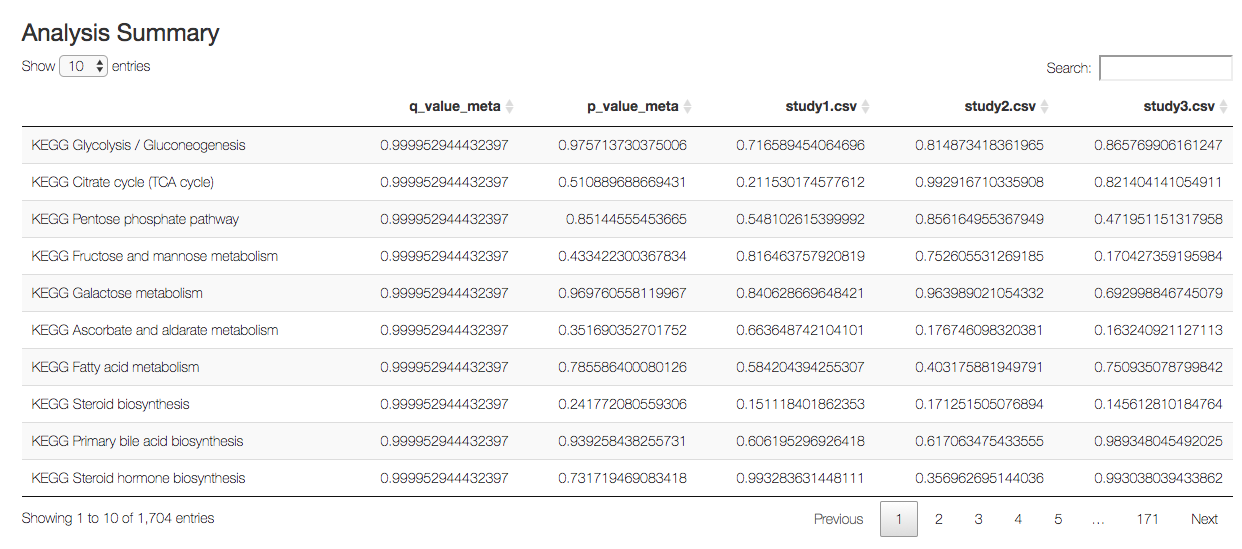
\includegraphics[scale=0.4]{./figure/metaPath/metaPathresult1.png}
\caption{MetaPath analysis summary. 
This table shows analysis results of all pathways, 
including individual study association analysis p-value, meta pathway analysis p-value/FDR, etc. 
Users can sort these pathways by clicking the p\_value\_meta ``up arrow" button.
In addition, users can search the pathway  name in the search bar.
}
\label{fig:MetaPathresult1}
\end{center}
\end{figure}

We used the AML data to demonstrate the usage of the MetaPath module
with the same filtering criteria and the phenotype of interest as in the MetaDE module.
Detailed descriptions of these studies can be found in Table~\ref{tab:realDataLeukemia}. 
After \ref{step:metaPath1} is finished, a summary table was generated, 
as shown in Figure~\ref{fig:MetaPathresult1} (based on the CPI method). 
The full table is automatically saved in the working directory specified previously.  

\begin{figure}[H]
\begin{center}
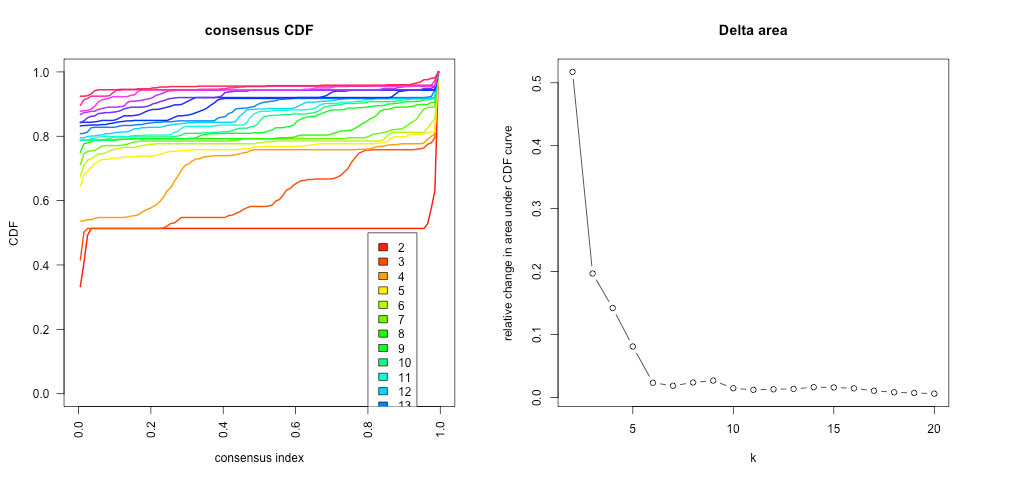
\includegraphics[scale=0.5]{./figure/metaPath/metaPathresult2.png}
\caption{MetaPath results (2).
Both plots assist users in finding the optimal number of clusters $K$, 
and users may refer to \cite{monti2003consensus} for detailed interpretation of the two plots. 
To be brief, the cumulative density function (CDF) of the consensus matrix for each $K$ (indicated by colors) is estimated by a histogram of 100 bins. 
The CDF reaches an approximate maximum, 
implying consensus and cluster confidence is at a maximum at this $K$. 
The Delta area shows the relative change in area under the CDF curve comparing $K$ and $K - 1$, thus allowing users to determine $K$ at which there is no appreciable increase in CDF (which drops as the number of cluster increases).
In the example, $K=5$ is chosen since it locates at the elbow turning point (i.e., where the magnitude of incremental decrease in delta area diminishes).
}
\label{fig:MetaPathresult2}
\end{center}
\end{figure}

In order to perform pathway clustering analysis, 
the number of clusters $K$ needs to be determined. 
By clicking ``Pathway Cluster Diagnostics" (\ref{step:metaPath2}), 
a user generates two plots on the right panel (Figure \ref{fig:MetaPathresult2}), 
including a consensus CDF plot and a Delta area plot (both from the ``ConsensusClusterPlus" package). 
Note that in this specific example, we set the FDR cutoff value in \ref{step:metaPath2} as 0.4, 
and 27 pathways are left under this cutoff.
Both plots assist users in finding the optimal number of clusters $K$, 
and a brief explanation is described in Figure~\ref{fig:MetaPathresult2}.
Users may refer to \cite{monti2003consensus} for a detailed interpretation of the two plots. 


\begin{figure}[H]
\begin{center}
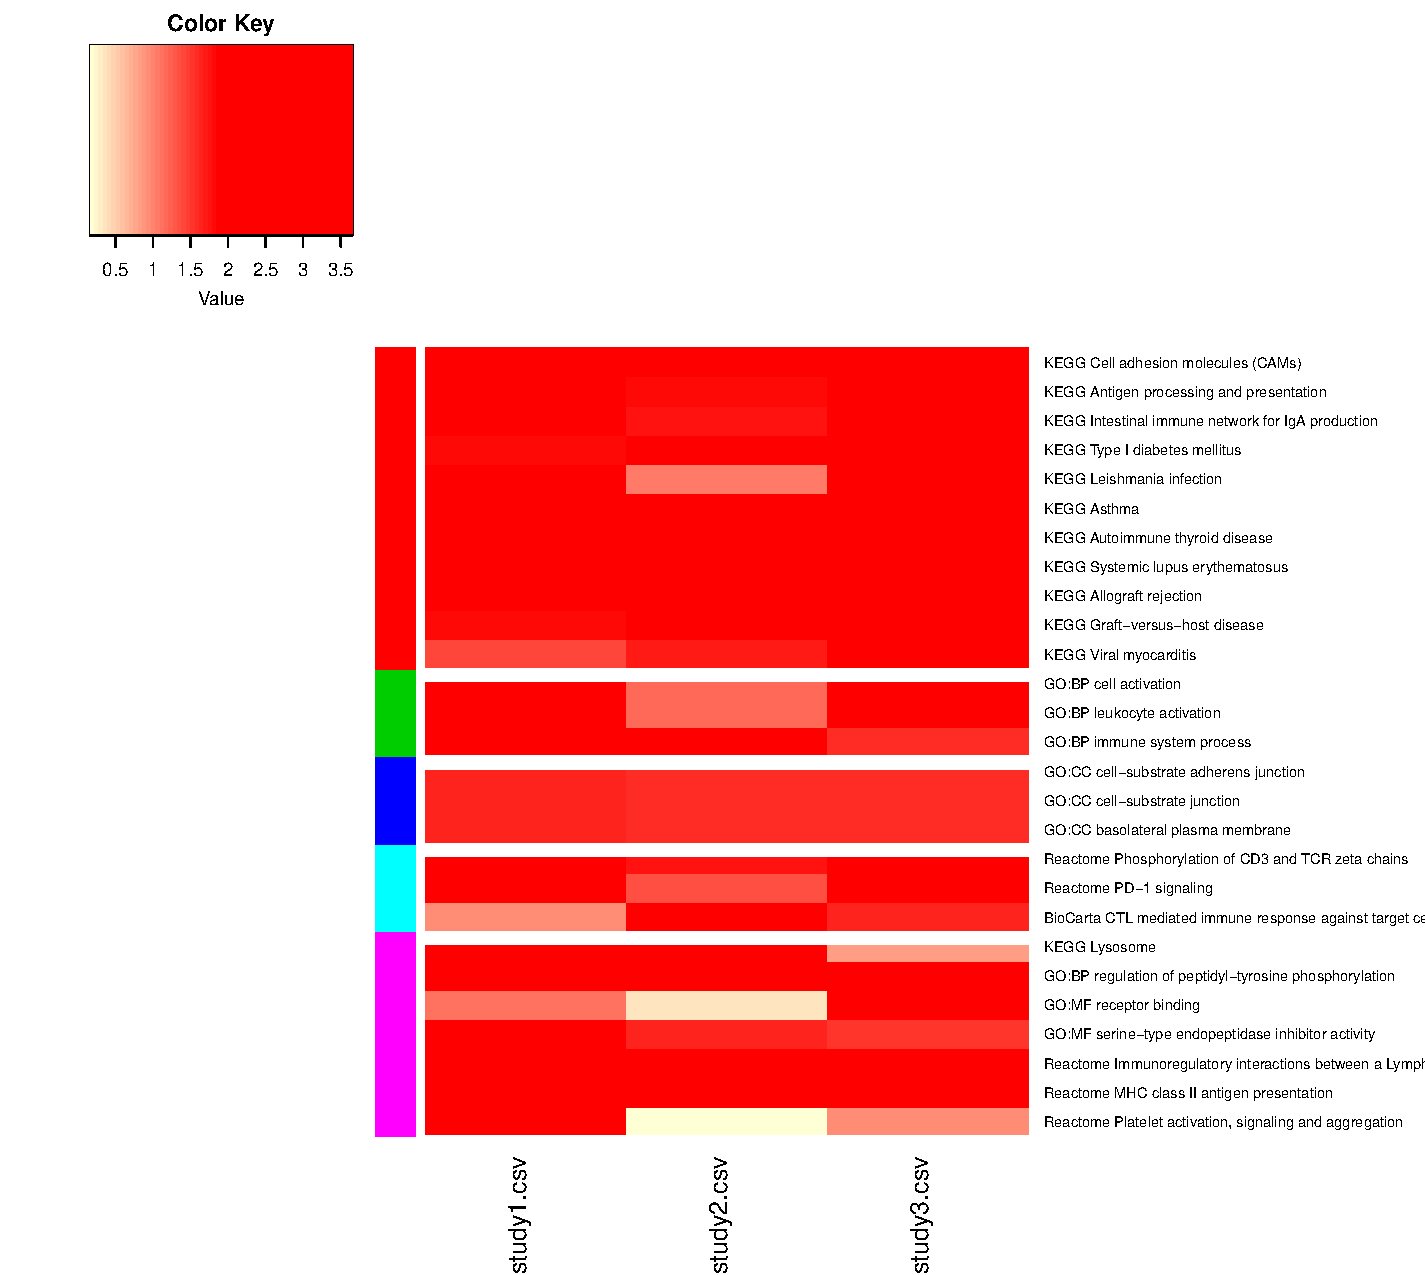
\includegraphics[scale=0.6]{./figure/metaPath/Heatmap_clusters_all.pdf}
\caption{MetaPath results (3).
The heatmap in Figure~\ref{fig:MetaPathresult3} shows the -log10 transformed p-value of enrichment analysis in each study from \ref{step:metaPath3}. 
Studies are on columns, 
and the selected pathways are on rows. 
The color bar on left indicates group of pathways.
In the heatmap, red indicates ``more enriched," 
and yellow  indicates ``not significantly enriched." 
The color key is on the top left corner. 
The pathways are sorted by the pathway clusters, 
as indicated by the colors on the left side of the heatmap.}
\label{fig:MetaPathresult3}
\end{center}
\end{figure}


The heatmap in Figure~\ref{fig:MetaPathresult3} shows the -log10 transformed p-value of enrichment analysis in each study from \ref{step:metaPath3}. 
In addition, 
key words of each cluster of pathways are extracted and analyzed by a built-in text mining algorithm. 
One file named ``Clustering\textunderscore Summary.csv" is saved to the working directory, 
which shows a summary of the text-mining results. 


